\documentclass[../sparc.tex]{subfiles}
\graphicspath{{\subfix{../images/}}}
\begin{document}

%%%%%%%%%%%%%%%%%%%%%%%%%%%%%%%%%%%%%%%%%%%%%%%%%%%%%%%%%%%%%%%%%%%%%%%%%%%%%%%%
\section{Working with a Breadboard}

\newglossaryentry{IDE}{name=IDE, description={Integrated Development
    Environment}}

A breadboard allows us to build electric circuits without using any soldering --
this makes prototyping easier and speeds up the process of project development.
Components can be just inserted in the sockets on the breadboard for connecting
them in the desired circuit (see fig. \ref{fig:breadboard-led}.)

\begin{figure}[ht]
  \centering
  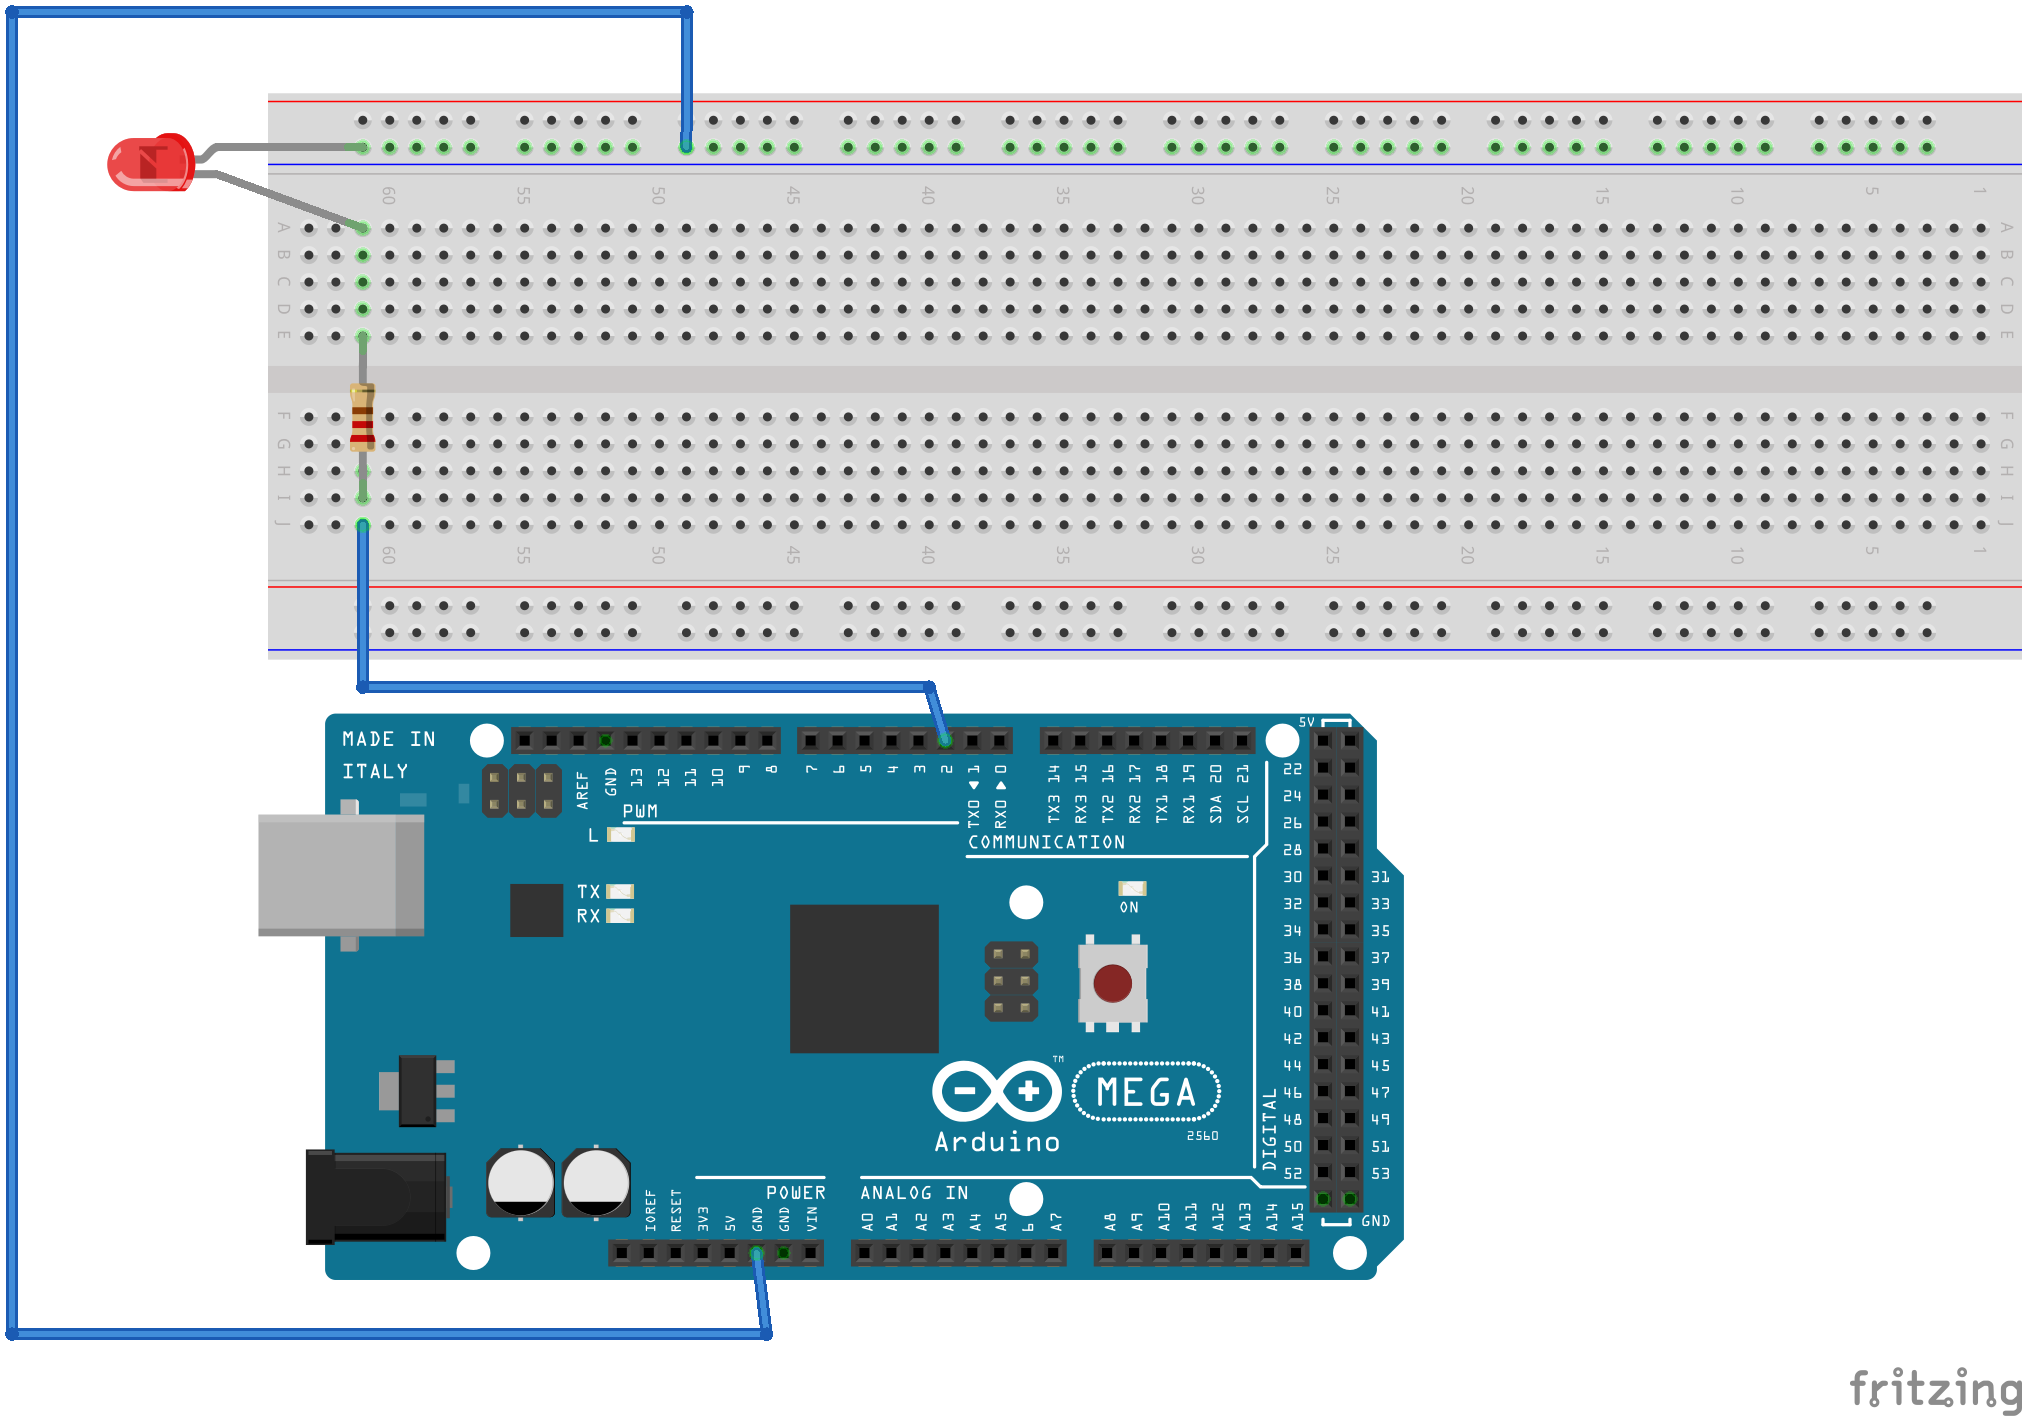
\includegraphics[width=12cm]{schematics/001-led}
  \caption{An example of a connection of a LED to Arduino Mega 2560 through the
    breadboard.}
  \label{fig:breadboard-led}
\end{figure}

\begin{itemize}
\item The black wire is connected to the Arduino GND pin.
\item The blue wire is connected to the Arduino 5V pin.
\end{itemize}

\note{ Note that LEDs and some other components are usually connected to an
  Arduino platform through a resistor -- as was discussed in section
  \ref{section:electronics-resistance} a resistor allows us to limit the current
  in a circuit thus protecting electronic components from premature failures. }

\section{Connecting an Arduino to a Computer}
To connect an Arduino board to a computer you'll need the board itself (in most
of our examples we will use Arduino Mega 2560) and a USB-B standard cable.

Connect the Arduino board to a computer using the USB-cable.  You should see
that the ``ON'' LED is light up on the board.

Now we need to configure our Arduino \gls{IDE} for working with your version of
the Arduino board.  To do that we need to open ``Tools'' in the window menu and
there open ``Boards'' sub-menu -- here we need to select the Arduino board model
that you're using right now.  Then we need to open ``Tools'' again and in
``Port'' sub-menu select the serial port to which your Arduino is connected.

\end{document}
